% !TEX root = ../main.tex

\chapter{PyTOD-FlashANNS 融合检测模型与数据准备}

\section{金融异常检测任务建模}

金融大规模异常检测任务的本质，是在高维、多源、强时序的交易与行为数据中，快速识别少量偏离正常模式的高风险样本。与一般的二分类任务不同，金融异常检测既受到标签稀缺、样本极度不平衡等问题的影响，也受到系统吞吐、响应时延和资源约束的直接限制\citep{aggarwal2017outlier,zhao2022tod}。在工程实现层面，系统必须能够同时处理原始交易记录、账户行为统计、设备与地理位置特征、时间窗口统计量以及可能存在的图结构关系。因此，本文首先对金融异常检测任务进行统一建模，以明确系统输入、候选召回目标、异常评分目标和输出形式，为后续 PyTOD--FlashANNS 融合框架设计奠定基础。

从输入形式上看，本文将待检测对象抽象为一个由样本集合 $X=\{x_1,x_2,\ldots,x_n\}$ 组成的金融行为数据集，其中每个样本 $x_i$ 对应一条交易记录、一个账户时间窗行为摘要或一个节点行为表示。每个样本由连续型数值特征、离散型类别特征和时间上下文特征组成，在预处理阶段被统一映射为固定维度向量表示 $v_i\in\mathbb{R}^d$。对于图结构金融数据，还需将节点特征与边关系经时间窗统计、邻域聚合或嵌入映射后转换为向量化表示，从而与表格型交易数据形成统一输入接口\citep{dgraphfin_paper,dgraphfin_baseline}。这一抽象使本文系统可以统一处理交易级异常、账户级异常以及图节点级异常，而不必为不同数据形式分别构建独立执行链路。

从系统目标上看，本文的异常检测任务并非直接对全量数据执行精确评分，而是采用``候选召回---异常评分''两阶段处理框架。第一阶段利用高吞吐近似最近邻检索在大规模样本中快速找到与查询样本最相关的候选集合 $C_i$，从而避免在全体样本上进行高代价比较；第二阶段利用 PyTOD 在候选集合上执行张量化异常评分，生成异常分数 $s_i$。形式上，可将系统目标写为
\begin{equation}
  C_i = \mathcal{R}(v_i, \mathcal{I}), \qquad s_i = \mathcal{F}(v_i, C_i),
\end{equation}
其中 $\mathcal{R}$ 表示候选召回过程，$\mathcal{I}$ 表示候选索引，$\mathcal{F}$ 表示异常评分函数。该二阶段处理结构使候选召回质量与异常评分质量共同决定最终检测效果，也使系统能够在大规模场景下获得更高吞吐率与更低资源开销\citep{zhao2022tod,xiao2025flashanns}。

从输出形式上看，系统可产生三类结果：其一是每个样本的异常分数，用于后续阈值判断或人工复核排序；其二是 Top-$k$ 风险样本集合，用于构造重点审查名单；其三是与异常结果相关的候选邻域、关键特征统计及日志信息，用于系统追踪和后续解释分析。对于金融风控场景而言，这三类结果分别对应在线筛查、风险排序和审计追踪三种实际需求。因此，本文后续设计的 PyTOD--FlashANNS 融合系统，不仅追求更高的候选召回吞吐和异常评分效率，也强调输出结果能够支持实验可重复性和工程可观察性。

图~\ref{fig:fin-ad-model} 对这一统一任务建模过程进行了整体展示，表~\ref{tab:task-io-def} 则进一步归纳了研究对象、输入表示与输出形式之间的对应关系。

\paragraph{图表预留说明：}
\begin{itemize}
  \item \textbf{图 3-1 金融异常检测任务建模图。} 展示交易数据、账户行为、图节点特征等不同输入形式如何统一映射为向量表示，并进入候选召回与异常评分两阶段流程。
  \item \textbf{表 3-1 研究对象、输入形式与输出形式定义表。} 列出交易级异常、账户级异常、图节点级异常三类对象，以及对应的输入字段、向量表示形式和输出结果类型。
\end{itemize}

\begin{figure}[htbp]
  \centering
  \thesisplaceholderbox{正式版补齐图~3-1}
  \caption{金融异常检测任务建模图}
  \label{fig:fin-ad-model}
\end{figure}

\begin{table}[htbp]
  \caption{研究对象、输入形式与输出形式定义}
  \label{tab:task-io-def}
  \centering
  \thesisplaceholderbox[0.95\linewidth]{正式版补齐表~3-1}
\end{table}

\section{实验数据集选取与构建}

本文的实验数据安排遵循``真实/半真实数据用于有效性验证，合成扩展数据用于系统吞吐与扩展实验''的基本原则。其原因在于：一方面，公开可获取的真实金融数据规模通常有限，且多经过脱敏、压缩或竞赛裁剪，适合验证模型与系统在现实场景中的可用性，但不足以单独支撑超大规模系统实验；另一方面，大规模性能验证需要控制数据规模、异常比例和字段分布的一致性，因此需要借助高保真合成数据集构建 10M 与 100M 规模实验环境\citep{ibm_aml_data,ibm_amlsim}。基于这一考虑，本文将实验数据集分为两类：第一类为 1M 规模的真实或半真实公开数据集，用于验证候选召回与异常评分在现实数据上的有效性；第二类为 10M 与 100M 规模的高保真合成数据集，用于验证系统在高吞吐与多 GPU 扩展场景下的性能表现。

在 1M 规模的有效性验证中，本文主要使用三类真实或半真实公开数据。第一类为 \textbf{IEEE-CIS Fraud Detection} 数据集，该数据集包含交易表与身份表两部分，特征维度高、缺失值复杂，较接近现实支付风控场景，可用于检验系统在高维结构化金融数据上的向量化表示与候选召回效果\citep{ieee_cis_fraud}。第二类为 \textbf{Credit Card Fraud Detection} 数据集，该数据集虽规模相对较小，但具有经典性和广泛使用基础，可作为基准异常检测数据集用于对照验证\citep{dalpozzolo2015creditcard}。第三类为 \textbf{DGraphFin} 金融图数据集，其包含大规模节点与边关系以及金融行为特征，适用于验证系统在图金融数据经过向量化映射后的可用性\citep{dgraphfin_paper,dgraphfin_baseline}。在具体实验组织时，本文将控制单次实验输入规模在约 1M 量级，以保证实验设计的一致性和可比较性。

在 10M 与 100M 规模的性能验证中，本文采用基于 \textbf{IBM AML / AMLSim} 体系构建的高保真合成金融交易数据。IBM AML-Data 明确以洗钱与异常金融交易为目标，提供带标签的合成金融交易数据集；AMLSim 则能够根据预定义行为规则、账户关系和交易模式生成大规模、可控分布的银行交易数据\citep{ibm_aml_data,ibm_amlsim}。本文利用该类数据的优势，在保持交易字段、行为模式、异常比例和实体关系结构相对稳定的前提下，将数据规模扩展至 10M 和 100M，以支撑候选召回吞吐、多 GPU 扩展和 I/O 路径压力测试。选择 IBM AML / AMLSim 而非简单随机生成数据的原因在于：其数据具有更强的金融语境和结构一致性，能够更真实地反映账户、交易和异常模式之间的关系，从而使系统性能结论更具工程意义\citep{ibm_aml_data,ibm_amlsim}。

除主实验数据外，本文还将利用数据集间的差异性补充分析系统的适用范围。具体而言，IEEE-CIS 与 Credit Card Fraud Detection 更适合检验结构化表格数据下的向量化表示与评分链路；DGraphFin 更适合验证系统在图金融数据上的扩展潜力；IBM AML / AMLSim 则主要用于高规模、高并发和多 GPU 扩展实验。通过这种``真实/半真实 + 合成扩展''的组合，本文在保证现实意义的同时，也为大规模并行系统验证提供了稳定实验基础。

为便于说明不同数据集在全文中的角色分工，表~\ref{tab:datasets-overall} 汇总了数据来源与基本属性，图~\ref{fig:dataset-scale-plan} 给出了规模层级安排，表~\ref{tab:dataset-roles} 对各数据集所支撑的实验任务进行了对应说明。

\paragraph{图表预留说明：}
\begin{itemize}
  \item \textbf{表 3-2 实验数据集总体信息表。} 表中列出各数据集的来源、类型、样本规模、特征维度、标签形式以及在本文中的用途。
  \item \textbf{图 3-2 数据集规模层级安排图。} 展示 1M、10M、100M 三个规模层级与对应数据集来源之间的关系，用于说明实验设计的逻辑。
  \item \textbf{表 3-3 数据集用途分工表。} 列出各数据集分别服务于有效性验证、单卡性能验证、多 GPU 扩展验证、图场景补充验证等任务。
\end{itemize}

\begin{table}[htbp]
  \caption{实验数据集总体信息}
  \label{tab:datasets-overall}
  \centering
  \thesisplaceholderbox[0.95\linewidth]{正式版补齐表~3-2}
\end{table}

\begin{figure}[htbp]
  \centering
  \thesisplaceholderbox{正式版补齐图~3-2}
  \caption{数据集规模层级安排图}
  \label{fig:dataset-scale-plan}
\end{figure}

\begin{table}[htbp]
  \caption{数据集用途分工}
  \label{tab:dataset-roles}
  \centering
  \thesisplaceholderbox[0.95\linewidth]{正式版补齐表~3-3}
\end{table}

\section{数据预处理与特征构造}

由于不同数据集在字段命名、数据类型、缺失值比例、标签分布以及时间粒度上存在较大差异，原始金融数据无法直接输入候选召回和异常评分模块。因此，在 PyTOD--FlashANNS 融合系统中，数据预处理与特征构造构成了统一系统输入表示的基础。本节的目标并不是对不同数据集设计完全不同的特征工程，而是在保证业务语义基本保留的前提下，将表格型金融数据和图结构金融数据统一映射为可检索、可评分的向量表示 $v_i\in\mathbb{R}^d$。

对于表格型金融数据，预处理过程主要包括缺失值处理、异常字段清洗、数值归一化、类别编码以及时间字段规范化。缺失值处理方面，针对数值型字段采用均值、中位数或业务合理缺省值进行填补，针对类别型字段则引入专门的缺失标识，以防止信息泄漏。异常字段清洗包括删除重复样本、去除明显无意义标识列、统一金额和时间单位等。对于数值型特征，本文采用标准化或归一化处理，减少金额、频率、时差等不同尺度特征之间的量纲影响；对于类别型字段，则采用 one-hot、频次编码或目标统计前的安全编码方式，以便后续统一映射至数值空间\citep{ieee_cis_fraud,dalpozzolo2015creditcard}。经过上述处理后，表格型交易记录能够以统一向量形式进入后续候选召回阶段。

对于时间信息，本文采用滑动时间窗和行为统计相结合的方式构造增强特征。具体而言，以单个账户、设备或商户为中心，在固定时间窗口内统计交易频次、交易金额分布、平均时间间隔、夜间交易比例、跨地域交易切换次数等行为特征，并将其与原始交易字段拼接形成更完整的查询表示。这样做的原因在于，单笔交易的异常性往往不仅由其当前字段决定，还受到历史行为模式的约束。通过时间窗统计，系统能够在不引入过于复杂序列模型的前提下，将部分时序上下文编码进向量表示，增强后续近邻候选召回与异常评分对行为模式的敏感性。

对于图金融数据，本文不直接在原始图结构上执行复杂图学习算法，而是先将图节点与边关系转换为节点级向量表示。具体做法包括：对节点原始属性进行规范化与编码；对邻域中边的数量、方向、金额统计和时间分布等进行聚合；将节点本身属性与邻域统计特征拼接形成统一向量。这样处理的目的在于，使 DGraphFin 等图金融数据能够与表格型交易数据共同进入本文统一的候选召回---异常评分链路\citep{dgraphfin_paper,dgraphfin_baseline}。

在最终特征构造阶段，本文将不同来源的特征统一组织为固定维度向量表示，并确保其满足两项要求：一是能够作为候选检索模块的输入，被 FAISS-GPU 或 FlashANNS 索引所接收；二是能够作为 PyTOD 评分主干的输入，参与距离计算、候选排序和异常评分。为此，本文在特征构造后执行一次统一的向量维度检查、类型检查与异常值截断，保证后续系统执行过程的稳定性和一致性。通过这一设计，本文将原本异构的金融数据源统一映射为候选召回与异常评分共同接受的输入形式，从而为后续融合执行流程提供基础。

图~\ref{fig:preprocess-overall} 展示了统一预处理链路，表~\ref{tab:feature-engineering} 细化了原始字段与派生特征之间的关系，图~\ref{fig:graph-vectorization} 则说明图金融数据如何映射到与表格数据兼容的节点向量表示。

\paragraph{图表预留说明：}
\begin{itemize}
  \item \textbf{图 3-3 数据预处理总体流程图。} 展示原始交易/图数据到规范化、编码、时间窗统计、向量表示生成的全过程。
  \item \textbf{表 3-4 特征构造明细表。} 列出原始字段、派生字段、特征类型、预处理方式及其在系统中的作用。
  \item \textbf{图 3-4 图金融数据向量化映射示意图。} 展示节点属性、边统计和邻域聚合如何转换为统一节点向量。
\end{itemize}

\begin{figure}[htbp]
  \centering
  \thesisplaceholderbox{正式版补齐图~3-3}
  \caption{数据预处理总体流程图}
  \label{fig:preprocess-overall}
\end{figure}

\begin{table}[htbp]
  \caption{特征构造明细}
  \label{tab:feature-engineering}
  \centering
  \thesisplaceholderbox[0.95\linewidth]{正式版补齐表~3-4}
\end{table}

\begin{figure}[htbp]
  \centering
  \thesisplaceholderbox{正式版补齐图~3-4}
  \caption{图金融数据向量化映射示意图}
  \label{fig:graph-vectorization}
\end{figure}

\section{PyTOD 异常评分主干设计}

在本文的两阶段异常检测框架中，PyTOD 承担的是候选集合上的异常评分主干角色。其作用并不是在全量样本上执行复杂评分，而是在候选召回阶段已经缩小搜索空间的前提下，对每个查询样本及其候选集合进行精细距离计算、近邻排序和异常性聚合，从而生成最终异常分数\citep{aggarwal2017outlier,zhao2022tod}。这种设计既保留了 PyTOD 在张量化执行和 GPU 评分上的优势，也避免了其在面对全量样本时所可能遭遇的显存和复杂度压力。

从方法学角度看，PyTOD 的核心优势在于能够将距离计算、排序、聚合和局部评分统一表示为张量算子组合\citep{zhao2022tod}。对于本文而言，这意味着候选集合 $C_i$ 一旦产生，查询样本 $v_i$ 与候选集合中的向量就可以直接进入 PyTOD 的计算链路中，被表示为批量距离矩阵、局部近邻排序结果与聚合统计结果。具体而言，本文在异常评分阶段主要执行以下几类操作：第一，计算查询样本与候选集合之间的距离；第二，对候选集合中的邻近样本按距离进行排序或筛选；第三，对局部距离分布、密度差异或邻域结构统计执行聚合；第四，根据预定义评分函数输出异常分数。与全量评分相比，这一路径显著缩小了 PyTOD 需要处理的样本范围，从而使其更适合作为大规模系统中的精排与评分组件。

在评分指标选择上，本文不局限于单一异常得分公式，而是保留基于距离、局部密度和邻域统计的通用评分接口。这一设计的原因在于，不同数据集和不同业务场景可能适合不同的异常性定义。由于 PyTOD 本身提供了统一张量算子组织能力，系统可以在不重构底层执行路径的前提下切换具体评分函数。因此，本文将 PyTOD 视为评分主干，而不是单一评分公式的固定实现。

需要特别说明的是，本文对 PyTOD 的使用方式与其原始``直接处理大规模全样本异常检测''的思路存在差异。TOD/PyTOD 更强调通过自动批处理和多 GPU 支持缓解全量异常检测的复杂度问题，而本文则通过候选召回模块先缩减样本范围，再在较小候选集合上执行 PyTOD 评分。这种调整并不是削弱 PyTOD，而是让其更适合本文所关注的近实时金融异常检测系统：一方面保留了其 GPU 异常评分能力，另一方面则将系统整体复杂度更多地转移到``候选召回 + 数据路径优化''这一更可控的层面。

图~\ref{fig:pytod-backbone} 给出了评分主干的执行流程，表~\ref{tab:score-ops-map} 对常用评分方式与张量算子映射进行了归纳，图~\ref{fig:full-vs-candidate} 则用于直观比较全量评分与候选集评分两条路径。

\paragraph{图表预留说明：}
\begin{itemize}
  \item \textbf{图 3-5 PyTOD 评分主干流程图。} 展示候选集合进入评分模块后，如何依次完成距离计算、局部排序、聚合统计与异常分数输出。
  \item \textbf{表 3-5 本文采用的异常评分指标与算子映射表。} 列出距离型、局部密度型和统计型评分方式，以及其对应的 PyTOD 张量算子链。
  \item \textbf{图 3-6 全量评分与候选集评分对比图。} 用于说明本文为何采用候选缩减后的评分路径。
\end{itemize}

\begin{figure}[htbp]
  \centering
  \thesisplaceholderbox{正式版补齐图~3-5}
  \caption{PyTOD 评分主干流程图}
  \label{fig:pytod-backbone}
\end{figure}

\begin{table}[htbp]
  \caption{异常评分指标与算子映射}
  \label{tab:score-ops-map}
  \centering
  \thesisplaceholderbox[0.95\linewidth]{正式版补齐表~3-5}
\end{table}

\begin{figure}[htbp]
  \centering
  \thesisplaceholderbox{正式版补齐图~3-6}
  \caption{全量评分与候选集评分对比}
  \label{fig:full-vs-candidate}
\end{figure}

\section{FlashANNS 候选召回模块设计}

在 PyTOD--FlashANNS 融合系统中，FlashANNS 负责从大规模样本中快速生成与查询样本最相关的候选集合，其目标不是输出最终异常结论，而是为后续精细评分阶段提供规模可控且质量可接受的候选近邻集合\citep{xiao2025flashanns}。这一模块的设计直接决定了后续 PyTOD 评分阶段的输入规模与局部邻域质量，因此其作用不仅体现在吞吐率上，也体现在系统最终检测效果的上界上。

在索引构建阶段，本文以向量化后的样本表示 $v_i$ 为输入，构建面向 ANN 检索的候选索引。对于规模较小且全部可驻留在显存内的实验场景，可直接使用 GPU 端索引完成近似搜索；对于规模更大或需要考虑外存路径的场景，则采用 FlashANNS 异步 I/O---计算流水线所支持的高吞吐检索路径\citep{xiao2025flashanns}。索引构建过程关注两个核心问题：一是保证查询时能够以低延迟定位到局部候选邻域；二是保证召回参数可调，以便在召回质量和系统吞吐之间进行平衡。

在查询执行阶段，FlashANNS 的作用是对输入查询向量 $v_i$ 快速检索并返回一个候选集合 $C_i$。在本文系统中，候选集合不仅包含候选 ID，还包含必要的距离值、局部排序信息或可支持后续评分的数据引用。之所以强调候选输出格式，是因为后续 PyTOD 评分阶段若仍需对候选结果做大量 CPU 侧整理与转换，则候选召回本身的吞吐收益会被显著削弱。因此，本文在设计候选召回模块时，特别强调其输出格式与评分模块输入接口的一致性，即尽量让候选结果以可直接进入 GPU 评分链路的形式表达。

在参数组织方面，本文通过控制候选集合规模、召回近邻数量和部分索引搜索参数，平衡候选召回质量与系统吞吐率。候选集合过小，可能导致真实异常邻域缺失，从而影响评分质量；候选集合过大，则会使后续 PyTOD 评分重新承受高复杂度负担。因此，本研究中候选召回模块并不追求极限检索精度，而是追求``对异常评分足够好''的候选质量。这种设计使候选召回模块能够作为服务于系统总体目标的前端组件，而不是独立优化指标的终点。

图~\ref{fig:flashanns-workflow} 展示了候选召回模块的基本执行过程，表~\ref{tab:recall-module-params} 总结了关键控制参数，图~\ref{fig:candidate-size-impact} 则说明候选集合规模对系统复杂度和后续评分负担的影响。

\paragraph{图表预留说明：}
\begin{itemize}
  \item \textbf{图 3-7 FlashANNS 候选召回执行流程图。} 展示索引构建、查询输入、候选返回和结果传递的基本流程。
  \item \textbf{表 3-6 候选召回模块主要参数表。} 包括候选数、近邻数、召回控制参数、候选输出字段等。
  \item \textbf{图 3-8 候选集合规模对系统复杂度影响示意图。} 展示候选集合过小、适中和过大对后续评分负担的影响。
\end{itemize}

\begin{figure}[htbp]
  \centering
  \thesisplaceholderbox{正式版补齐图~3-7}
  \caption{FlashANNS 候选召回执行流程图}
  \label{fig:flashanns-workflow}
\end{figure}

\begin{table}[htbp]
  \caption{候选召回模块主要参数}
  \label{tab:recall-module-params}
  \centering
  \thesisplaceholderbox[0.95\linewidth]{正式版补齐表~3-6}
\end{table}

\begin{figure}[htbp]
  \centering
  \thesisplaceholderbox{正式版补齐图~3-8}
  \caption{候选集合规模对系统复杂度影响示意图}
  \label{fig:candidate-size-impact}
\end{figure}

\section{PyTOD--FlashANNS 融合执行流程}

在完成数据预处理、向量化表示、候选召回模块和异常评分主干设计后，本文将二者整合为统一的执行流程。该流程覆盖从查询输入到异常结果输出的完整链路，其核心目标是在保持模块职责清晰的同时，减少阶段间不必要的数据复制和格式转换。具体而言，系统的整体执行过程包括以下五个步骤。

第一步，系统接收原始交易记录、账户行为摘要或图节点样本，并将其经过第三节所述的数据预处理与特征构造过程转换为统一向量表示。第二步，向量表示作为查询输入候选召回模块，由 FlashANNS 或与之协同的 GPU ANN 检索后端从大规模样本索引中返回候选集合。第三步，候选集合在 GPU 侧完成必要的组织与重排，使其能够直接作为 PyTOD 评分主干的输入。第四步，PyTOD 在候选集合上执行张量化异常评分，输出异常分数及对应排序结果。第五步，系统根据异常分数输出风险样本、日志记录和必要的解释信息，并进入后续实验采样或部署监控链路。

该融合执行流程的关键，不在于``把两个模块接起来''，而在于两者之间的中间结果表达与执行边界设计。若候选召回结果必须回传 CPU 再被整理成评分输入，则系统链路会重新引入高昂的 CPU$\leftrightarrow$GPU 往返与阶段同步成本；若中间结果能够以 GPU 常驻张量或低开销设备对象表达，则整个``候选召回---异常评分''过程将更接近统一 GPU 执行链路。也正因此，本文在第三章虽然主要完成逻辑模型构建，但已经明确后续第四章的核心方向：进一步将融合流程从``功能可行''压缩为``数据路径低开销''。

图~\ref{fig:fusion-pipeline} 总结了融合系统的整体阶段划分，图~\ref{fig:intermediate-dataflow} 进一步展示查询向量、候选结果与评分中间张量在模块间的传递方式，表~\ref{tab:module-interfaces} 则对接口字段与数据驻留位置进行了统一定义。

\paragraph{图表预留说明：}
\begin{itemize}
  \item \textbf{图 3-9 PyTOD--FlashANNS 融合执行总流程图。} 展示输入、预处理、候选召回、候选组织、异常评分、结果输出六个阶段。
  \item \textbf{图 3-10 模块间中间结果传递示意图。} 展示查询向量、候选结果和异常评分中间张量的流转方式，用于为第四章单卡数据路径优化做铺垫。
  \item \textbf{表 3-7 模块接口定义表。} 列出输入格式、输出格式、主要字段和数据驻留位置。
\end{itemize}

\begin{figure}[htbp]
  \centering
  \thesisplaceholderbox{正式版补齐图~3-9}
  \caption{PyTOD--FlashANNS 融合执行总流程图}
  \label{fig:fusion-pipeline}
\end{figure}

\begin{figure}[htbp]
  \centering
  \thesisplaceholderbox{正式版补齐图~3-10}
  \caption{模块间中间结果传递示意图}
  \label{fig:intermediate-dataflow}
\end{figure}

\begin{table}[htbp]
  \caption{模块接口定义}
  \label{tab:module-interfaces}
  \centering
  \thesisplaceholderbox[0.95\linewidth]{正式版补齐表~3-7}
\end{table}

\section{基础实验与初步验证}

在进入系统级优化和多 GPU 扩展之前，有必要首先验证 PyTOD--FlashANNS 融合流程在功能上的正确性和在 1M 量级数据上的基本可用性。因此，本节以真实或半真实 1M 规模数据为基础，围绕以下三个问题开展基础实验：第一，候选召回与异常评分链路是否能够正确联通；第二，在候选集合上执行 PyTOD 评分是否会造成不可接受的检测效果损失；第三，融合流程在初始实现下是否已具备进一步开展系统优化的基础。

在功能正确性验证中，实验主要关注查询输入、候选集合生成、候选组织与异常评分输出之间是否存在接口不一致、结果异常或批处理错误。对于 1M 规模数据，本文通过抽样检查、异常分数排序和标签对照等方式验证系统链路的稳定性。随后，通过将候选评分结果与小规模全量评分结果进行比较，分析候选召回对异常评分效果的影响。如果候选集合过小导致异常模式无法被覆盖，则说明候选召回参数仍需调整；如果候选评分与全量评分在主要排序结果上具有较高一致性，则说明两阶段框架具备继续系统优化的基础。

基础实验还将初步观察不同数据集下候选召回与异常评分之间的关系。例如，结构化交易数据中的候选召回结果往往对金额、时间和设备行为更敏感，而图金融数据中的候选召回结果则更容易受到邻域统计特征影响。通过这种初步实验，本文能够在进入第四章和第五章之前，先确认 PyTOD--FlashANNS 融合路线在不同金融数据形态下都具有基本可行性。

表~\ref{tab:basic-exp-setup} 给出了基础实验配置，图~\ref{fig:recall-vs-full-consistency} 用于验证候选评分与全量评分之间的一致性，图~\ref{fig:prelim-effectiveness} 则展示了不同数据集上的初步有效性结果。

\paragraph{图表预留说明：}
\begin{itemize}
  \item \textbf{表 3-8 基础实验设置表。} 包括数据集、输入规模、候选数量、评分参数和实验目标。
  \item \textbf{图 3-11 候选召回与全量评分一致性对比图。} 用于展示两阶段框架在基础场景下的可行性。
  \item \textbf{图 3-12 不同数据集上的初步有效性结果图。} 用于展示结构化交易数据与图金融数据上的初步表现。
\end{itemize}

\begin{table}[htbp]
  \caption{基础实验设置}
  \label{tab:basic-exp-setup}
  \centering
  \thesisplaceholderbox[0.95\linewidth]{正式版补齐表~3-8}
\end{table}

\begin{figure}[htbp]
  \centering
  \thesisplaceholderbox{正式版补齐图~3-11}
  \caption{候选召回与全量评分一致性对比}
  \label{fig:recall-vs-full-consistency}
\end{figure}

\begin{figure}[htbp]
  \centering
  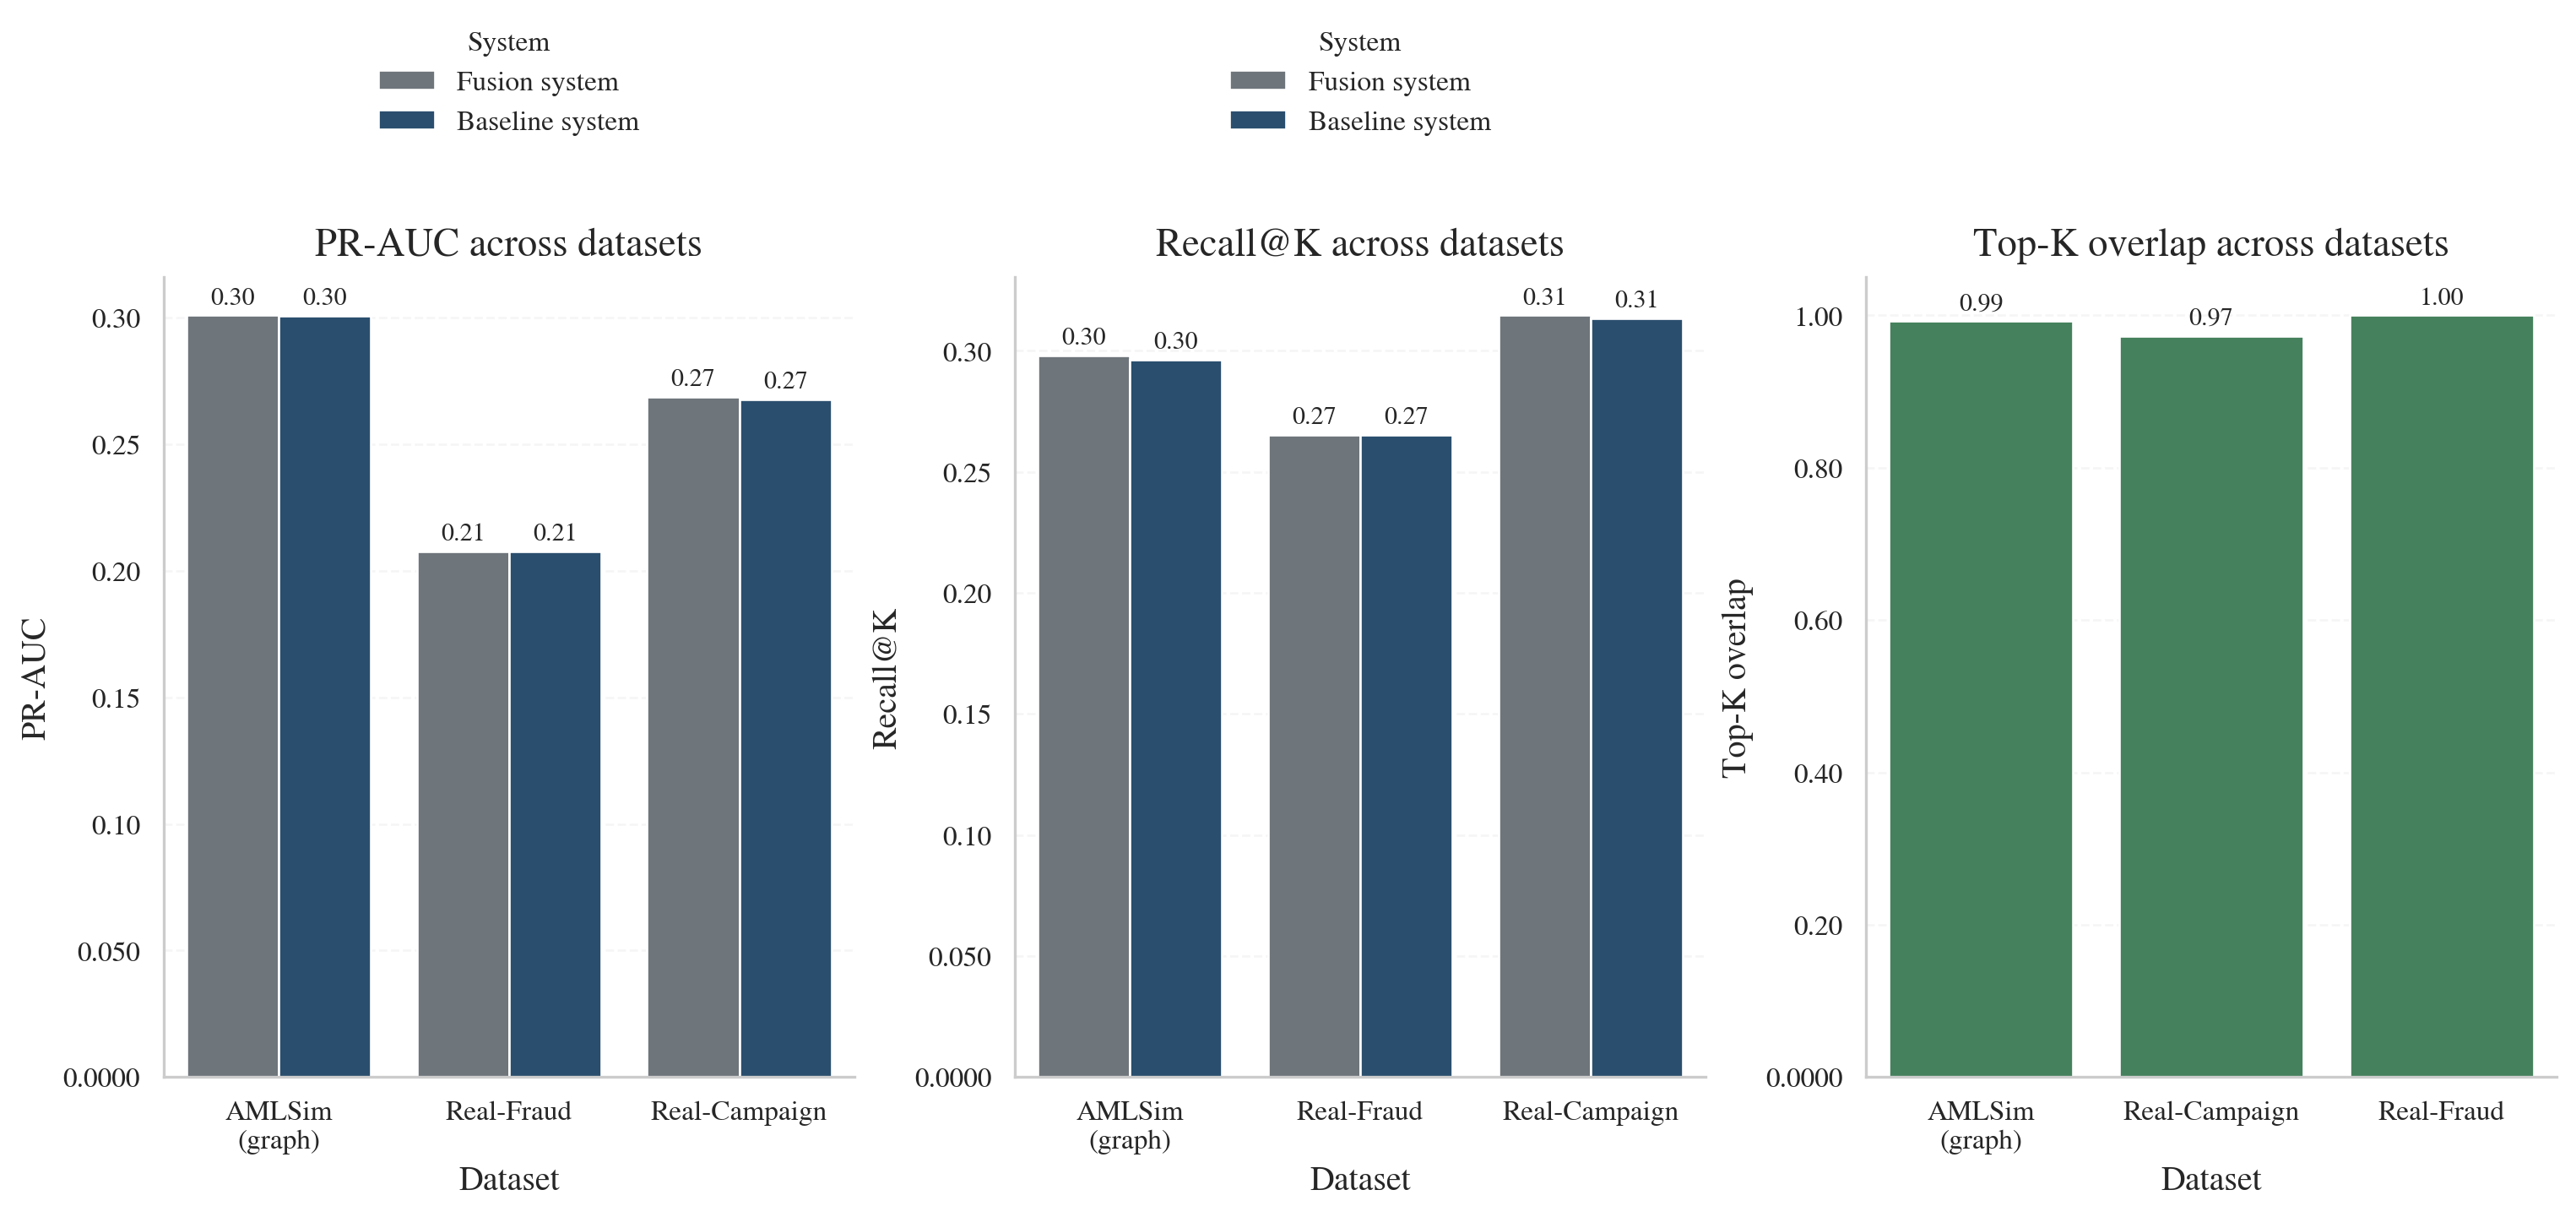
\includegraphics[width=\linewidth]{figures/fig_3_12_initial_effectiveness_across_datasets.png}
  \caption{不同数据集上的初步有效性结果}
  \label{fig:prelim-effectiveness}
\end{figure}

\section{本章小结}

本章围绕 PyTOD--FlashANNS 融合系统的功能结构，完成了任务建模、数据集选取、预处理与特征构造、异常评分主干设计、候选召回模块设计以及融合执行流程构建。通过对金融异常检测任务的统一抽象，本文将表格型金融数据与图金融数据共同映射为向量表示，并建立了``候选召回---异常评分''的两阶段处理框架。在数据集安排上，本文明确采用真实/半真实数据进行 1M 规模有效性验证，采用高保真合成数据进行 10M 与 100M 规模系统吞吐和扩展实验，从而为后续章节中的单卡优化和多 GPU 验证提供了数据基础\citep{ibm_aml_data,ibm_amlsim,dgraphfin_baseline}。

更重要的是，本章并未把 PyTOD 与 FlashANNS 视作两个孤立模块，而是将它们统一放置在一条候选召回---异常评分执行链路中加以考察。基础实验表明，该融合路线在功能上是可行的，但在当前阶段仍然主要解决``能否工作''的问题，尚未从系统层面彻底压缩数据路径和阶段同步开销。因此，下一章将在本章流程设计的基础上，进一步从单卡场景出发，重点研究 GPU 主导的端到端执行链路、异步 I/O---计算流水线与数据路径压缩问题\citep{xiao2025flashanns}。


